\documentclass[journal]{IEEEtran}
\interdisplaylinepenalty=2500

\usepackage{array}
\usepackage{graphicx}
\usepackage{epsf}
\usepackage{float}
\usepackage{stfloats}
\usepackage[font=footnotesize]{caption}
\usepackage[font=footnotesize]{subcaption}
\usepackage{cite}
\usepackage{picinpar}
\usepackage{siunitx}

\usepackage{amsmath, nccmath}
\usepackage{url}
\usepackage{flushend}
\usepackage{colortbl}
\usepackage{soul}
\usepackage{multirow}
\usepackage{pifont}
\usepackage{color}
\usepackage{alltt}
\usepackage[hidelinks]{hyperref}
\usepackage{enumerate}
\usepackage{siunitx}
\usepackage{breakurl}
\usepackage{epstopdf}
\usepackage{pbox}


\usepackage{booktabs}
\usepackage{wrapfig}

\graphicspath{{../}}

\usepackage{placeins}
\usepackage{latexsym}
\usepackage{amssymb}
\usepackage{xifthen}
\usepackage{balance}
\usepackage{multicol}
\renewcommand{\arraystretch}{1.2}




\newenvironment{conditions}
  {\par\vspace{\abovedisplayskip}\noindent\begin{tabular}{>{$}l<{$} @{${}-{}$} l}}
  {\end{tabular}\par\vspace{\belowdisplayskip}}


\ifCLASSINFOpdf

\else
 
\fi


\hyphenation{op-tical net-works semi-conduc-tor}


\begin{document}

\title{Analysis and DSP Implementation of Multisampled Three-Phase Current Controllers}


% make the title area
\maketitle

\begin{abstract}
nothing yet
\end{abstract}

% Note that keywords are not normally used for peerreview papers.
\begin{IEEEkeywords}
nothing yet
\end{IEEEkeywords}


\IEEEpeerreviewmaketitle

\section{Introduction}
\IEEEPARstart{F}{ield} oriented control (FOC) in electrical drives and voltage oriented control (VOC) in grid-connected converters is a well-established strategy for the control of high performance three-phase electrical systems \cite{holmes2012}. An essential part of this concept is the inner current control loop, which regulates the synchronous rotating frame (SRF) currents \cite{holmes2009}. A prerequisite for the proper operation of the outer control loops is a precise and rapid current controller ~\cite{yepes2014,choi1998}. The SRF controller must provide a decoupling function between d and q axis currents []. This is particularly challenging for high-speed or high pole-pair electrical drives, which require robustness at very high output frequencies ~\cite{choi1998,hoffmann2016,yim2009}. 

Due to simplicity and added flexibility, current controllers are nowadays mostly realized in digital form [Buso Matta]. The demerit of digital control systems is the introduction of delays due to the analog-to-digital conversion (ADC), algorithm execution time, and digital pulse width modulation (DPWM) [Buso Matta]. These delays limit the achievable bandwidths and impair the decoupling function of SRF current controllers. 
In most state-of-the-art applications, double-sampled double-update (DS-DU-PWM) control strategy is used, where the inductor currents are sampled twice per PWM period, with acquisition instants being synchronized so that average current values are obtained []. In industrial applications, feedback signal is often strongly corrupted by various noise sources, which requires additional filtering []. This is well-achieved by oversampling the signal and then averaging it over the PWM period. In this way, true-average is obtained with additional high noise suppression. The filtered signal is then decimated so that the control action is executed with double-update rate. This kind of strategy, implemented in \cite{vuksa2016}, is labeled as multi-sampled double-update (MS-DU-PWM) control. The MS-DU-PWM strategy results in a high quality feedback signal, however, with a highly negative impact on the system dynamics. Achieving high bandwidths with the additional delay due to the averaging requires modification of the controller structure to compensate the phase lag due to averaging [].

The delay-related limitations have inspired investigating multisampled PWM control, with purpose of enabling analog-like control bandwidths in digital systems. The multisampled multi-update (MS-MU-PWM) approach relies on acquiring the control variables and updating the modulating waveform multiple times per switching period \cite{corradini_analysis}. The concept of MS-MU-PWM digital control offers significant reduction of digital delays and is therefore a promising solution for breaking the bandwidth limitations \cite{corradini2018} [MS in electric drives]. Besides small-signal improvement, MS-MU-PWM has always additional nonlinear advantage that is obtained with the capability of modifying the modulating waveform multiple times per switching period. This is important for large-signal disturbance rejection [active filtering]. On the other hand, MS-MU-PWM introduces a set of nonlinearities due to sampling of the switching ripple, which is why some digital filtering should always be implemented ~\cite{petric2020,petric2021}. The impact of nonlinearities is strongly reduced by completely filtering the switching ripple, for example using moving average filters (MAFs).

Regarding controller structures, SRF PI controllers are the most frequently encountered current control strategies for three-phase $RL$ loads due to their simplicity and satisfactory performance for the majority of the industry requirements ~\cite{rowan1986,bae2003,yepes2014}. With a proper parameter setting procedure, high bandwidths can be achieved ~\cite{yepes2014,holmes2009}. Nevertheless, their transient decoupling capability is rather limited, especially at high output frequencies \cite{lorenz2000}. Achieving robust operation with high bandwidths has driven the design of high-performance current controllers directly in discrete-time domain \cite{bae2003} [lorenz...]. The dead-beat current controllers offer very fast transient response but at the cost of considerable performance degradation in the presence of measurement errors and parameter mismatch, which is often the case in control of electric drives ~\cite{malesani1999,xu2019,rovere2018}. More robust operation is achieved with the use of the discrete internal model controller (IMC) design \cite{lorenz2010}. This strategy has proven to offer high closed loop bandwidths at very high output frequencies ~\cite{commentsHoffmann,vuksa2016,petric2021a}.

This paper analyzes the use of the discrete IMC based current controller with MS-MU-PWM, suitable for implementation on standard DSP platforms. The main goal of the paper is to analyze the performance of MS-MU-PWM in standard industrial applications, and to compare it with standardly used DS-DU-PWM and MS-DU-PWM methods. 
%The MS-PWM control strategy is analyzed for three different control loop organizations. The first one uses discrete IMC controller from \cite{vuksa2016}, with a moving average filter (MAF) in the feedback. This case is found to offer slightly improved dynamics compared to standard use of double-update with the same discrete IMC (without filter in feedback) ~\cite{lorenz2010,vuksa2016}, with significant improvement in jitter suppression. Due to added delays introduced by the MAF, the second case adds a derivative action to the controller structure, as in \cite{vuksa2016}. This case is given to demonstrate that MS-PWM can offer even better dynamics than reported in \cite{vuksa2016}. The final case implements MS-PWM based discrete IMC, without any filters in feedback. This case is expected to provide the best dynamics, using discrete IMC without derivative gain. The feedback quality is expected to worsen compared to cases with MAFs, hower, it still retains higher quality compared to double-update \cite{petric2020}. 
The target is to show that the MS-MU-PWM control with feedback averaging can offer high quality feedback signal as in MS-DU-PWM, while also providing improved dynamic performance compared to DS-DU-PWM. This gives potential of implementing MS-MU-PWM with feedback averaging as standard industrial procedure for current control.

%This paper is organized as follows. Section II addresses discrete time machine model, controller structure and analyzes delays introduced by feedback averaging, calculation and DPWM. The multisampling PWM approach, with an outline of its merits and demerits, is explained in Section III. A DSP implementation of the multisampling algorithm is also presented. Exact controller structures and parameter setting procedures for the three aforementioned cases of interest are derived in Section IV. Effectiveness of the derived analytical model is illustrated via simulated current loop step responses and frequency response analyses. Comparison between performance of the proposed methodology and benchmark controllers is also provided. Experimental results are shown in section V. Conclusions are drawn in section VI, along with a proposal for further studies on the presented topic.
 
\section{Multi-rate control system}

\begin{figure*}[t!]
    \centerline{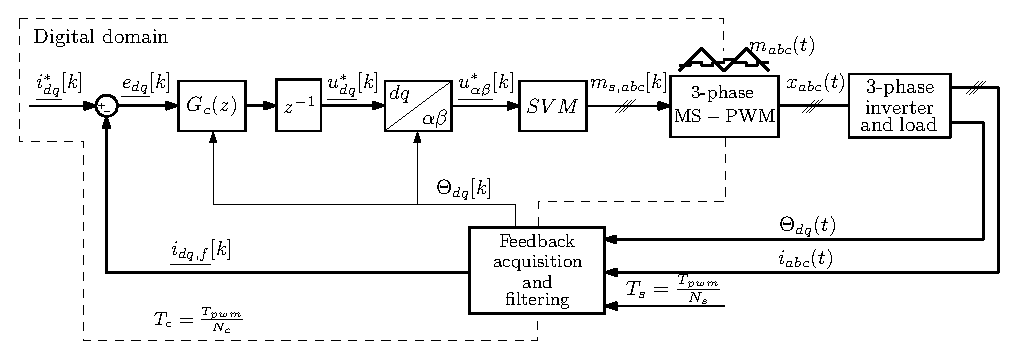
\includegraphics[width=0.95\linewidth]{figures/schematic.eps}}
    \caption{Multisampled control loop of a three-phase inverter.}
    \label{fig:MSControl}
\end{figure*}

The multi-rate control system of a three-phase $RL$ load in $dq$ frame is shown in Fig. 1. The system can be separated into digital and continuous-time domain. An ADC is used to transform feedback signal from analog to digital domain. This action is performed with a sampling frequency $f_s = N_s f_{pwm}$, where $N_s$ is the multisampling (oversampling) factor and $f_{pwm}$ is the switching frequency of the inverter. The digital domain operates with frequency $f_c = N_c f_{pwm}$, where $N_c$ is the multi-update factor that determines the update rate of the controller output. The choice of this frequency is independent of the sampling frequency, as the feedback signal can be oversampled with frequency $f_s$ and then filtered and decimated to control frequency $f_c$. The digital domain is comprised of feedback filter $G_{fb}(z)$, controller $G_c(z)$, coordinate frame transformation block, and space vector modulation (SVM) block. The controller $G_c(z)$ outputs reference voltage in $dq$ frame, $\underline{u_{dq}}^*[k]$, which is then transformed to $\alpha \beta$ frame. This reference voltage is used to obtain digital modulating waveform for each inverter phase, $m_{s,abc}[k]$. Conversion from digital to analog domain is performed by MS-PWM. Its inherent zero-order hold function transforms the digital impulse train $m_{s,abc}[k]$ into the continuous-time modulating waveform $m_{abc}(t)$. MS-PWM with the triangular carrier is used due to its favorable characteristics in MS-MU-PWM control []. The PWM output is used as a gate signal $x_{abc}(t)$. The three-phase inverter is used to supply the $RL$ load, which can be an AC electrical machine or electrical grid. The sensed feedback includes line currents $i_{\alpha \beta}(t)$ and the angle of the $dq$ coordinate frame $\Theta_{dq}$. 

\subsection{Motivation behind MS-MU-PWM control}

Modern processors feature high computational power, which enables short execution times for control routines. However, switching frequencies of power converters are hardware limited, and do not go over several tens of kHz for medium power applications. This hardware based limitation directly affects the realizable bandwidths of the current control loop, which subsequently limits the outer control loops. Therefore, pushing for highest possible bandwidths relative to the switching frequency is often a design criterion. One way of achieving that is the implementation of MS-MU-PWM [].

Using describing function approach, small-signal model of the multisampled PWM with triangular carrier is found to be almost equal to a pure delay of $\frac{T_c}{2}$, where $T_c$ is the modulating waveform update period []:

\begin{equation}
\begin{aligned}
G_{DPWM} (s) = \frac{d(s)}{m(s)} = A(\omega,D,N_c) e^{-s\frac{T_c}{2}},
\label{eq:DPWM} 
\end{aligned}    
\end{equation}
where $s$ is the complex variable of the Laplace transform, $d$ is the continuous-time duty cycle used for averaged modeling [], $\omega$ is the angular frequency, and $D$ is the steady-state duty cycle. The gain $A$ can be approximated with unity gain with negligible losses in modeling accuracy [].
In DSP applications, update of the modulating waveform is usually delayed by one control period $T_c$, due to the non-negligible computational time []. This update delay can be represented in s-domain as:

\begin{equation}
\begin{aligned}
G_{ud} (s) = e^{-sT_c}.
\label{eq:updateDelay} 
\end{aligned} 
\end{equation}

Combining delays due to modulation \eqref{eq:DPWM} and algorithm computation \eqref{eq:updateDelay} results in total digital delay being equal to:

\begin{equation}
\begin{aligned}
\tau_{d} = \frac{3}{2}T_c = \frac{3}{2} \frac{T_{pwm}}{N_c}
\label{eq:tauD} 
\end{aligned}    
\end{equation}

From \eqref{eq:tauD}, it can be seen that multi-update control reduces digital delays inversely proportionate to the multi-update factor $N_c$. Traditionally, double-update is the most often used method, which results in twice decreased delays compared to single-update.
Term multisampled (multi-update) control is most often used when $N_c$ is increased above 2. This kind of control is a promising way of bringing the digital control close to analog regarding achievable bandwidths []. However, care must be taken as significant nonlinearities are also introduced in the control system, mainly due to the discontinuity of the modulating waveform, which now features switching ripple component as well. For this reason, multi-update control is most often followed by feedback filtering, which entirely removes the switching ripple from the feedback signal []. 

\subsection{Discrete-time model of a three-phase RL load}

Given the simplicity of the inverter topology with a $RL$ load, its model can be easily derived directly in discrete-time domain, without the use of Tustin's method and transport delay approximations []. This kind of modeling is important for design of digital controllers, as it enables highest achievable bandwidths with inherent decoupling of $dq$ axes []. 
Note that for direct-discrete modeling, the action of the PWM is assumed to be equal to a zero-order hold in stationary $\alpha \beta$ frame []:
\begin{equation}
\begin{aligned}
G_{DPWM,\alpha \beta} \approx \frac{1-e^{-sT_c}}{s}.
\label{eq:DPWMAlphaBeta} 
\end{aligned}    
\end{equation}
 This is true for the case of single- and double-update PWM, however, for $N_c>2$, the exact model is shown in \eqref{eq:DPWM}. For the very specific case of triangular carrier, MS-PWM can still be well-approximated with a ZOH with update rate equal to $f_c$, specially regarding its phase response [].

The direct discrete-time modeling can be found in [lorenz2010,vukosavic2016,DOI 10.1109/TPEL.2018.2841206]. This paper follows the procedure from [DOI 10.1109/TPEL.2018.2841206].
In order to analyze the three-phase $RL$ load as single-input single-output (SISO) system, complex variables are used []. 
Starting from $\alpha \beta$ frame differential equations necessary for modeling are:

\begin{equation}
\begin{aligned}
\underline{u}_{\alpha \beta} (t) = R \underline{i}_{\alpha \beta} (t) + L \frac{d}{dt} \underline{i}_{\alpha \beta} (t),
\label{eq:alphaBetaVoltage} 
\end{aligned}    
\end{equation}
where $R$ and $L$ are the line resistance and the line inductance, respectively. The machine back-emf or the grid voltage is neglected in this analysis, as the paper focuses purely on enhancing the current-loop response, without taking into account disturbance rejection.
The s-domain transfer function from applied voltage to the line current, corresponding to \eqref{eq:alphaBetaVoltage} is:

\begin{equation}
\begin{aligned}
G_{i,\alpha \beta} = \frac{1}{R} \frac{1}{1 + s \frac{L}{R}}.
\label{eq:sDomainAlphaBeta} 
\end{aligned}    
\end{equation}


Multiplication of \eqref{eq:updateDelay}, \eqref{eq:DPWMAlphaBeta} and \eqref{eq:sDomainAlphaBeta} yields the plant model in $\alpha \beta$ frame.
The transformation from $\alpha \beta$ to $dq$ frame is obtained using the substitution $s \rightarrow s + j \omega_o$, where $\omega_o$ is the $dq$ frame rotating frequency.
This yields the following s-domain plant transfer function in $dq$ frame:

\begin{equation}
\begin{aligned}
G_{p,dq}(s) = e^{-s T_c} e^{-j\omega_o} \frac{1-e^{-sT_c}e^{-j\omega_oT_c}}{s+j\omega_o} \frac{1}{R} \frac{1}{1 + s \frac{L}{R} + j\omega_o \frac{L}{R}}.
\label{eq:modelSdomain} 
\end{aligned}    
\end{equation}
 
The discrete-time model is obtained directly from \eqref{eq:modelSdomain} using $\mathcal{Z}$ transform table:

\begin{equation}
\begin{aligned}
G_{p,dq}(z) = \frac{\left( 1 - e^{-\frac{R}{L}T_c}\right) e^{-2j\omega_o T_c}}{R} \frac{1}{z \left( z - e^{- \left( \frac{R}{L} + j\omega_o\right) T_c}\right)},
\label{eq:modelZdomain} 
\end{aligned}    
\end{equation}
where $z$ is the complex variable of the $\mathcal{Z}$ transform.

The model obtained in \ref{eq:modelZdomain} is used for the subsequent derivation of the model-based controller.
 
\subsection{Discrete IMC controller}


\begin{figure}[t!]
    \centerline{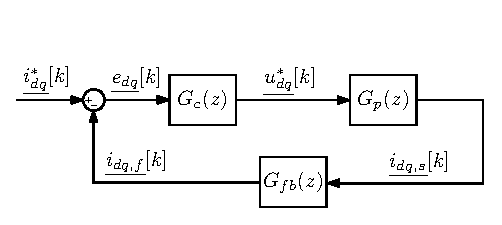
\includegraphics[width=0.95\linewidth]{figures/small_signal.eps}}
    \caption{Small-signal block diagram of the system from Fig. \ref{fig:MSControl} in discrete-time domain.}
    \label{fig:SmallSignal}
\end{figure}

The $dq$ frame discrete-time small signal block diagram of the control system in Fig. \ref{fig:MSControl} is shown in Fig. \ref{fig:SmallSignal}. In this paper, IMC method is used to obtain the controller structure []. The goal of the method is to inverse the plant model with addition of an integrator with gain $\alpha$ that determines the crossover frequency []. For the sake of causality, due to digital delays, additional factor of $\frac{1}{z^2}$ is added to the controller structure, which results in the following transfer function:

\begin{equation}
\begin{aligned}
G_{c}(z) =  \frac{\alpha \cdot z}{z-1} \frac{1}{z^2} G^{-1}_{p,dq}(z)  =   \frac{\alpha \cdot R \cdot e^{j\omega_o T_c}}{\left( 1 - e^{-\frac{R}{L}T_c}\right)}\frac{z e^{j\omega_o T_c}-e^{-\frac{R}{L}T_c}}{z-1}.
\label{eq:Controller} 
\end{aligned}    
\end{equation}

By implementing controller from \eqref{eq:Controller}, without any feedback filters, open-loop transfer function is obtained:

\begin{equation}
\begin{aligned}
W_{ol,1}(z) = G_c(z) G_p(z) =  \frac{\alpha}{z(z-1)}
\label{eq:OpenLoop} 
\end{aligned}    
\end{equation}

In [vukosavic] it is shown that relying on two samples per $T_{pwm}$ often results in unacceptable feedback signal deterioration in industrial applications. This is due to the unalignement between the voltage impulse and sampling instants due to limited current sensor bandwidths, analog feedback filters, delays in driver circuits, and similar. Furthermore, feedback signal often comprises oscillations due to the $LC$ parasitics of long cables that are present in industrial drives. This is a motivation behind the implementation of MS-DU-PWM in[] and MS-MU-PWM in this paper, where the signal is highly oversampled and then averaged over $T_{pwm}$.

\section{Feedback acquisition, coordinate frame transformation, and filtering}

\subsection{Feedback acquisition and $\alpha \beta - dq$ transformation}

The timing diagram of feedback acquisition, coordinate frame transformation and controller update is shown in Fig. \ref{fig:timings}. The modulating waveform is illustrated for one phase, $m_a(t)$.
The system analyzed in this paper features two independent discrete-time frequencies. First one is the control frequency, which defines the controller execution rate and update of the modulating waveform. It is defined by the multi-update factor $f_c = N_c f_{pwm}$. Control interrupts are synchronized with the carrier $w(t)$ such that two are always occurring at instants when carrier is equal to its maximum and zero value. Fig. \ref{fig:timings} is given for $N_c = 4$. At instant $k$, $dq$ frame feedback current $i_{dq,f}[k]$ is obtained and used to calculate the voltage reference $u^*_{dq}[k]$, which is used to calculate the segment of the modulating waveform that is applied at the beginning of the following control interrupt. As reported in [], $N_c$ should be chosen as the highest possible value allowed by the DSP processing power, in order to decrease the MS-PWM nonlinearities introduced by the discontinuities of the modulating waveforms. The synchronous frame signal $\Theta_{dq}$ is obtained each $T_c$ by implementing a PLL or using resolver/encoder sensors. 
The second frequency is the sampling frequency, which is defined by the multisampling factor $f_s = N_s f_{pwm}$. This factor allows the DSP to acquire the signal with much higher rate than it can calculate control algorithms, by employing standardly available DMA module. High sampling rates allow the subsequent use of digital filters, for example MAFs, to obtain a true average value each $T_c$ - $i_{dq,f}[k]$.


\begin{figure}[t!]
    \centerline{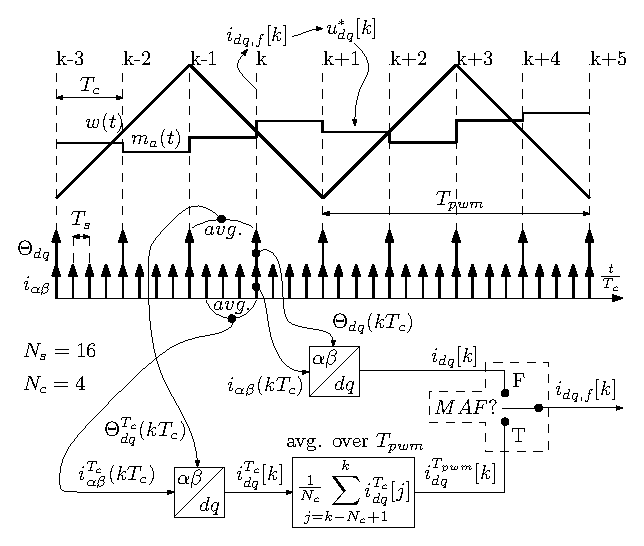
\includegraphics[width=0.95\linewidth]{figures/timing_diagram.eps}}
    \caption{nothing yet}
    \label{fig:timings}
\end{figure}

In case of DS-DU-PWM method, $N_c = N_s = 2$, $i_{\alpha \beta}[k]$ and $\Theta_{dq}[k]$ are used to obtain $i_{dq,f}[k]$. This is the standard control method, most-often used in the state-of-the-art digital current controllers []. 

In case of MS-DU-PWM methods, $N_c = 2$, $N_s>2$. This kind of feedback acquisition is analyzed in []. The factor $N_s$ is chosen to be as high as allowed by the maximal ADC sampling rate. At each control interrupt, package of $\alpha \beta$ frame currents is obtained via a DMA buffer, and averaged over $T_c$. This averaged current $\overline{i}_{\alpha \beta}[k]$ is transformed to $dq$ frame using the average value of $\Theta_{dq}[k]$ and $\Theta_{dq}[k-1]$. Finally, the resulting $dq$ frame current is filtered using MAF with the result from the previous interrupt to obtain feedback current averaged over the entire switching period, $\overline{i}_{dq}[k]$. 

Finally, for the case of MS-MU-PWM methods, the procedure is the same as for MS-DU-PWM methods, except that $N_s \geq N_c > 2$. For MS-MU-PWM methods, MAF can be used in the same manner as for MS-DU-PWM, in order to avoid introducing switching ripple into the control loop. This filtering is not always used for MS-MU-PWM, when highest dynamic performance is required []. However, for three-phase industrial drives, the effect of nonlinearities introduced by the modulating waveform discontinuities still needs to be investigated. 

For the purpose of later controller tuning, multi-rate system should be analyzed in a unique discrete-time domain, corresponding to the frequency $f_c$. For this reason, to avoid modified $\mathcal{Z}$ transform, MAF action can be closely analyzed using the following transfer function [vukosavic]:

\begin{equation}
\begin{aligned}
G_{MAF}(z) = \frac{1 + 2z^{-\frac{N_c}{2}} + z^{-N_c}}{4}.
\label{eq:MAF} 
\end{aligned}    
\end{equation}


\subsection{Total time delay in DSP application}

For control loop analysis and comparison between DS-DU-PWM, MS-DU-PWM, and MS-MU-PWM based on the crossover frequency and phase margin it is of interest to analyze loop delays in continuous-time domain.

The equivalent time delay of calculation and DPWM modulation is shown in \eqref{eq:tauD}. For DS-DU-PWM without any feedback filtering, this corresponds to the total delay:

\begin{equation}
\begin{aligned}
\tau_{d,DS-DU} = \frac{3}{2} \frac{T_{pwm}}{2}.
\label{eq:tauDSDU} 
\end{aligned}    
\end{equation}

For MS-DU-PWM, MAF is most often used [] to filter out the switching frequency component. The phase lag of the MAF over $T_{pwm}$ can be closely approximated by a pure delay equal to $\frac{T_{pwm}}{2}$ []. This results in the equivalent time-delay:

\begin{equation}
\begin{aligned}
\tau_{d,MS-DU,MAF} = \frac{3}{2} \frac{T_{pwm}}{2} + \frac{T_{pwm}}{2} = \frac{5}{4} T_{pwm}.
\label{eq:tauMSDU} 
\end{aligned}    
\end{equation}

For MS-MU-PWM without MAF, equivalent time-delay is equal to \eqref{eq:tauD}.
Finally, for MS-MU-PWM with MAF, equivalent time-delay is:
\begin{equation}
\begin{aligned}
\tau_{d,MS-MU,MAF} = \frac{3}{2} \frac{T_{pwm}}{N_c} + \frac{T_{pwm}}{2} = \frac{\frac{3}{N_c}+1}{2}T_{pwm}.
\label{eq:tauMSMUMAF} 
\end{aligned}    
\end{equation}

From above the following can be concluded. First of all, MS-DU-PWM features significant time-delay due to MAF and high modulating and control delays. This kind of feedback acquisition is indeed often necessary due to high deterioration of the signal quality in industrial drives []. However, for high dynamic performance, MS-DU-PWM controller structure needs to include additional derivative gain compared to \eqref{eq:Controller}, to compensate for the high delays. Regarding dynamics, best case represents MS-MU-PWM without MAF. With high multi-update factors $N_c \geq 8$ [], control delays are practically removed and dynamic capabilities approach analog control. This means that the achievable bandwidths are limited purely by PWM frequency. However, strong nonlinearities may exhibit due to the introduction of the switching ripple component 
Finally, from \eqref{eq:tauMSMUMAF} it can be seen that for MS-MU-PWM with a MAF, starting from $N_c>6$, equivalent time delay is reduced compared to DS-DU-PWM. This is important, as the same kind of filtering as in MS-DU-PWM is used, which results in a high quality feedback signal, while the dynamics is improved compared to traditionally used DS-DU-PWM. By filtering the switching ripple, high nonlinearities due to multi-update control are strongly attenuated. 
In the end, it should be mentioned that multi-update control always features additional nonlinear advantage compared to DU, as the reference voltage can be modified $N_c$ times per PWM period, which improves large-signal response of the controller. 

\section{Controller parameter design}
The aim of this section is to introduce different control loop architectures which will be compared in order to illustrate benefits of the proposed MS-MU-PWM methodology. Parameter setting procedure for each controller is also provided. IMC gains are set analytically using the plant and feedback models derived in Sections II and III. \par
The first tested strategy is the state-of-the-art DS-DU approach with IMC controller from \cite{vuksa2016}. IMC gain for this controller is set to the highest value which results in the step response without an overshoot \cite{vuksa2016}. Even though DS-DU strategy provides satisfactory dynamic performance in case of a high quality feedback signal, it may exhibit poor performance in presence of various noise sources, which is often the case in industrial applications [].  \par
Modification of the previously discussed control loop via an addition of oversampled MAF (MS-DU) in the feedback path eliminates sampling errors caused by the lock-out time and parasitic LC oscillations \cite{vuksa2016}. It however negatively impacts controller dynamic performance. In the analysis that will follow, IMC gain for this MS-DU controller is chosen so that the step response exhibits less than $1\%$ overshoot \cite{vuksa2016}. \par
Proposed MS-MU IMC controller with MAF based feedback acquisition is considered next. The goal is to show that with this control loop architecture, both DS-DU high-quality dynamic performance and MS-DU robust feedback acquisition can be achieved. IMC gain for the proposed controller is set so that similar cross-over frequency is achieved as in case of DS-DU controller. In this way delays introduced by feedback averaging in MS-DU approach are compensated, and phase margin is improved for $N>6$. \par
For the previously introduced controllers, IMC gains and analytically obtained cross-over frequencies and phase margins are shown in Table \ref{tab:an_param}. These results will be verified in the subsequent sections by means of simulation and experimental results.\par

\begin{table}[h!]
			  \caption{Control loop parameters}
              \label{tab:an_param}
              \centering
              \begin{tabular}{llll}
                           \midrule\midrule
        MS-MU+MAF & label & value   & unit\\
        \midrule               
                  IMC gain	& $\alpha$ & 0.0636 & /\\  
                  Cross-over frequency  & $f_{c}$ & 798.5845 & Hz   \\
                  Phase margin  & $pm$ & 70.2667 &  $^\circ$  \\
                  \midrule\midrule
        DS-DU & label & value   & unit\\
        \midrule               
                  IMC gain	& $\alpha$ & 0.25 & /\\  
                  Cross-over frequency  & $f_{c}$ & 799.1594 & Hz   \\
                  Phase margin  & $pm$ & 68.4572 &  $^\circ$  \\
                  \midrule\midrule
        MS-DU & label & value   & unit\\
        \midrule               
                  IMC gain	& $\alpha$ & 0.17 & /\\  
                  Cross-over frequency  & $f_{c}$ & 538.7873 & Hz   \\
                  Phase margin  & $pm$ & 65.7934 &  $^\circ$  \\
                  \midrule\midrule
                                                        
              \end{tabular}
\end{table}

\section{Simulation results}
\textbf{Ivan: The simulation results are not yet perfectly tuned. It will be done after we see what can we achieve in experiments.}
Performance of the previously introduced three control loop architectures is evaluated by means of computer simulations in MATLAB/Simulink. Results of the simulated step responses and open-loop frequency response analyses are provided. In addition to this, analytically obtained results are compared with those from simulation, with the aim of verifying modelling approach explained in Sections II and III. \par
Simulation is organized as follows. Current controller is modelled in discrete domain whereas all relevant delays are taken into account. Detailed model of DPWM, which resembles action qualifier module realization within DSP EPWM peripheral, is implemented. Load is modeled in continuous time domain using Simulink abc machine model. Simulation results presented in this section are obtained with BLDC motor from \cite{vuksa2016}. Switching frequency is set to 10kHz. For the proposed MS-MU controller, multi-update factor is set to eight, which was limited by the total execution time of the FOC algorithm. MAF, when used for the feedback acquisition, assumes averaging of 16 samples per switching period. Prior to sampling, motor currents are filtered using a first order low-pass filter with $\tau_{fil} = 5 \mu s$). \par
The dq current loop step responses, for the three previously discussed controllers, are simulated and compared to the step response of the closed loop transfer functions obtained via modelling approach described in Sections II and III. Simulations are run with the controller parameters from Table \ref{tab:an_param}. The results are shown in Fig. \ref{fig:MSMUmaf_step}-\ref{fig:MSDU_step}. Presented step responses are obtained at $270 Hz$ electrical frequency with $1 \mu s$ dead-time. A slight mismatch between the analytical and simulated MS-MU + MAF step responses exist, wheres DS-DU and MS-DU analytical and simulated results are in excellent agreement. No coupling between axis is present for either of the controllers. The derived plant model for the proposed MS-MU controller will be further examined via FRA simulation. \par
The same simulation model which is used to simulate step responses is used to perform FRA. However, when running FRA simulations  dead-time is set to $0$, so that non-linear effects which could mask FRA responses are avoided. Open loop FRA simulations are organized in the following manner. For the analyzed axis, sinusoidal perturbation of $0.1 A$ is used as an excitation signal. Error in the other axis is set to zero. The perturbation frequencies are an arithmetic sequence from $400 Hz$ to $5000 Hz$, with a step of $50 Hz$. Q axis open loop FRA results for the three control loop architectures of interest are shown in Fig. \ref{fig:MSMUmaf_olfra}-\ref{fig:MSDU_olfra}. Simulated results are compared to the analytically obtained ones. Summary of the simulation results is provided in Table \ref{tab:sym_param}. The results in Fig. \ref{fig:MSMUmaf_olfra} validate the derived control loop model, since mismatch between analytical and simulated waveforms is hardly noticeable and exists only in the higher frequency range. In addition to this, cross-over frequency and phase margin of the simulated MS-MU + MAF control loop are similar to those provided in Table \ref{tab:an_param}. When compared to DS-DU controller, MS-MU + MAF achieves the same cross over frequency and phase margin, which is as expected, taking into account parameter setting procedure used for the proposed controller. Therefore, the proposed MS-MU approach offers MAF based feedback acquisition without degrading control loop dynamic performance. In this way, the noise and sampling errors in the feedback path are successfully eliminated due to MAF based feedback acquisition as in MS-DU, but also the dynamic performance is kept as high as in case of state-of-the-art DS-DU controller. \par


\begin{figure}[t!]
    \centerline{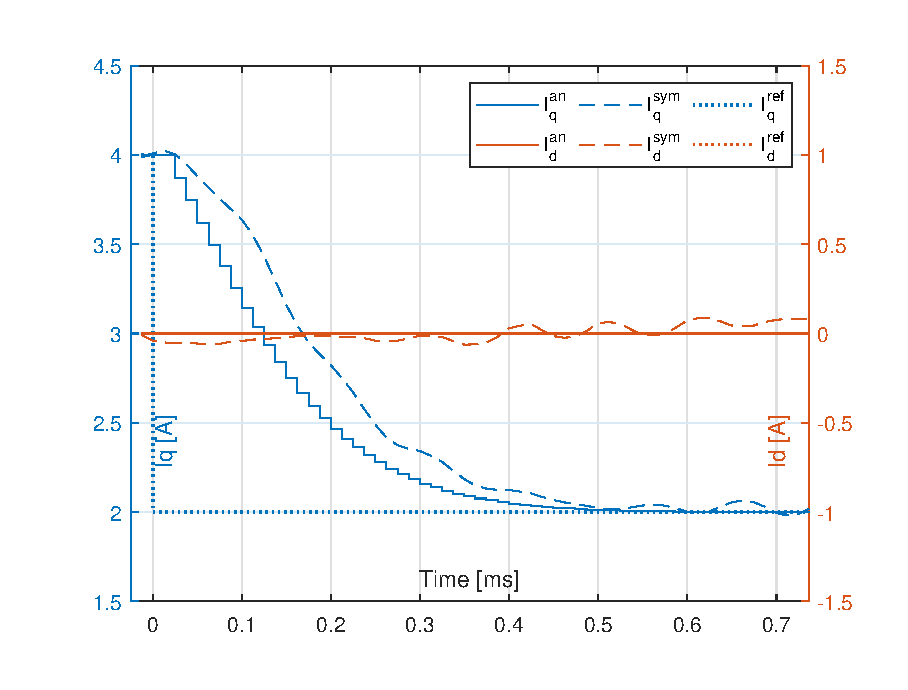
\includegraphics[width=0.95\linewidth]{figures/MSMUmaf_step.eps}}
    \caption{Simulated step response for MS-MU + MAF controller.}
    \label{fig:MSMUmaf_step} 
\end{figure}
\begin{figure}[t!]
    \centerline{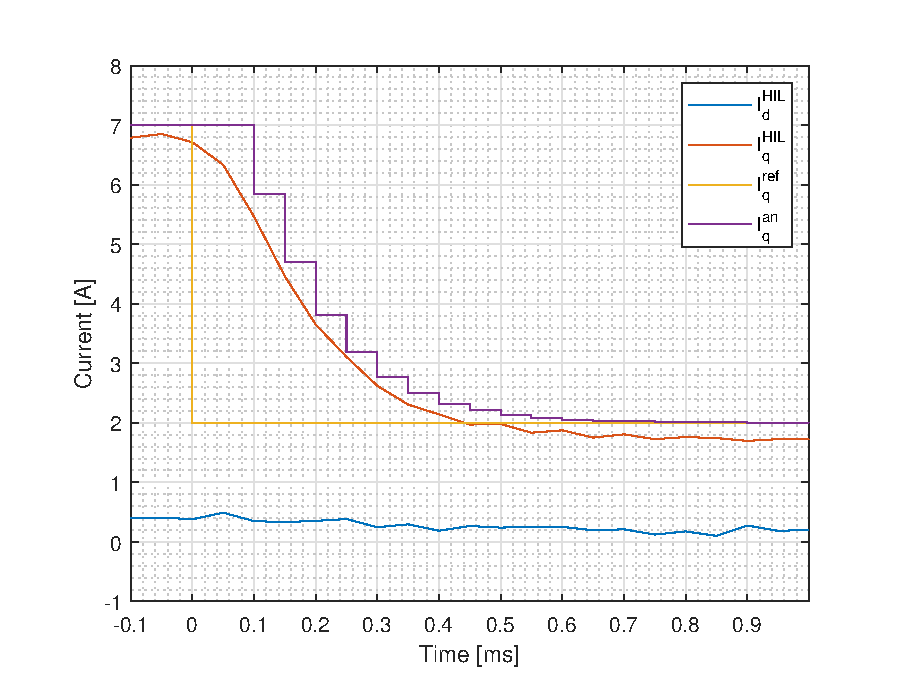
\includegraphics[width=0.95\linewidth]{figures/DSDU_step.eps}}
    \caption{Simulated step response for DS-DU controller.}
    \label{fig:DSDU_step} 
\end{figure}
\begin{figure}[t!]
    \centerline{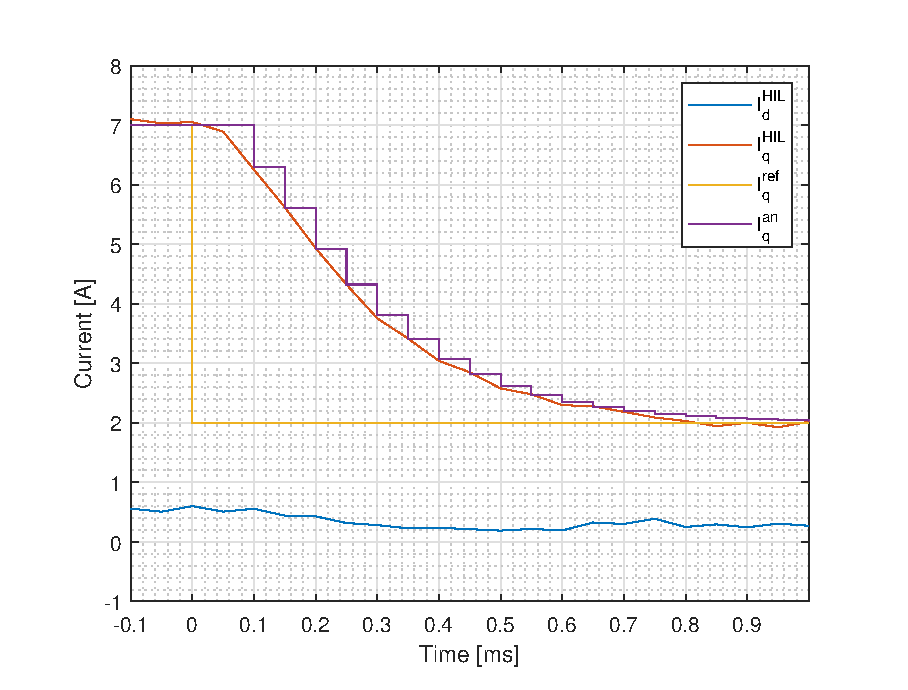
\includegraphics[width=0.95\linewidth]{figures/MSDU_step.eps}}
    \caption{Simulated step response for MS-DU controller.}
    \label{fig:MSDU_step} 
\end{figure}

\begin{figure}[t!]
    \centerline{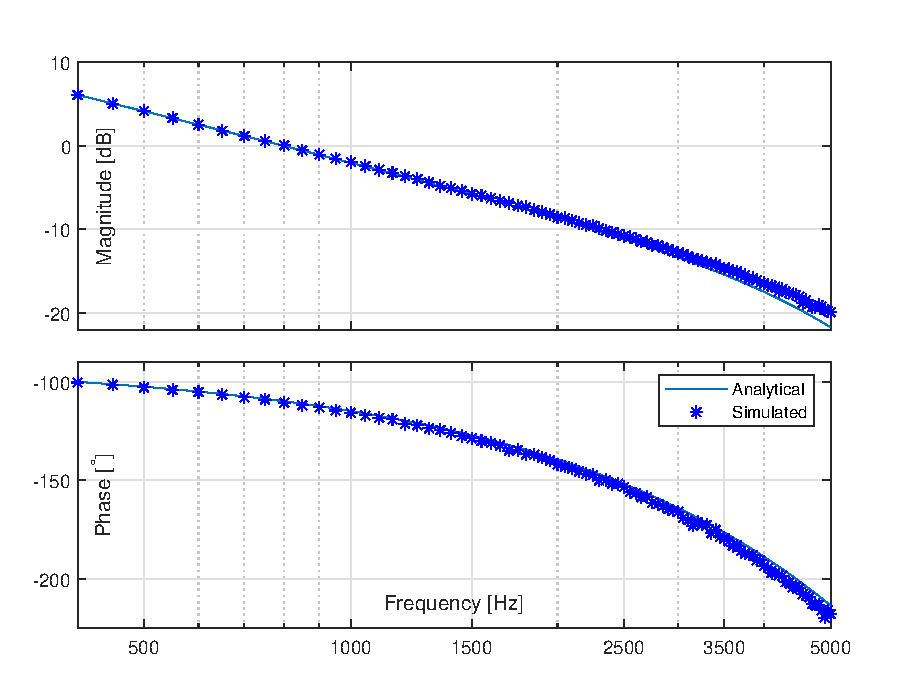
\includegraphics[width=0.95\linewidth]{figures/MSMUmaf_olfra.eps}}
    \caption{Simulated open loop FRA results for MS-MU + MAF controller.}
    \label{fig:MSMUmaf_olfra} 
\end{figure}
\begin{figure}[t!]
    \centerline{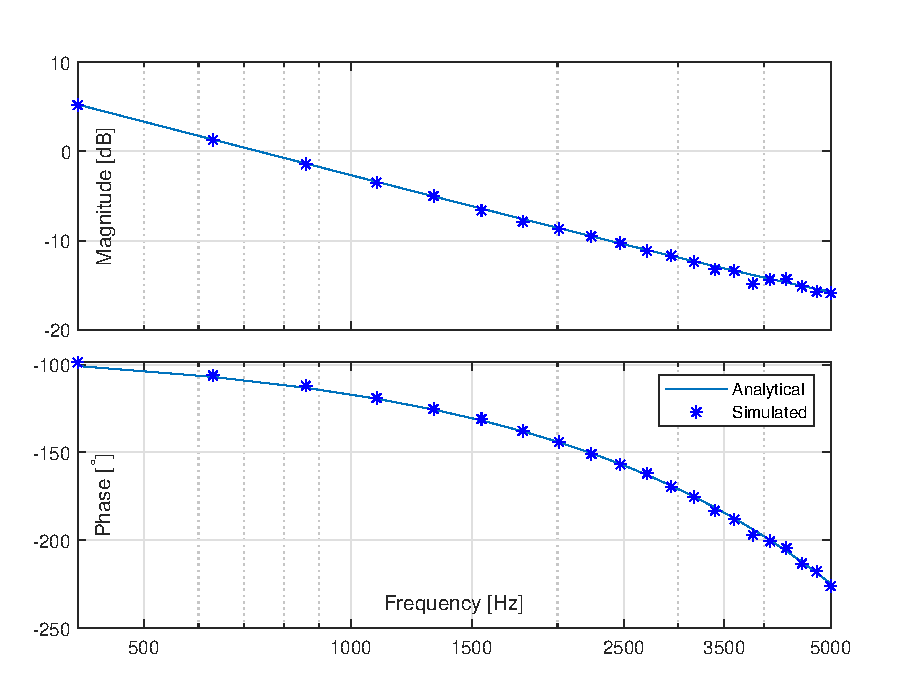
\includegraphics[width=0.95\linewidth]{figures/DSDU_olfra.eps}}
    \caption{Simulated open loop FRA results for DS-DU controller.}
    \label{fig:DSDU_olfra} 
\end{figure}
\begin{figure}[t!]
    \centerline{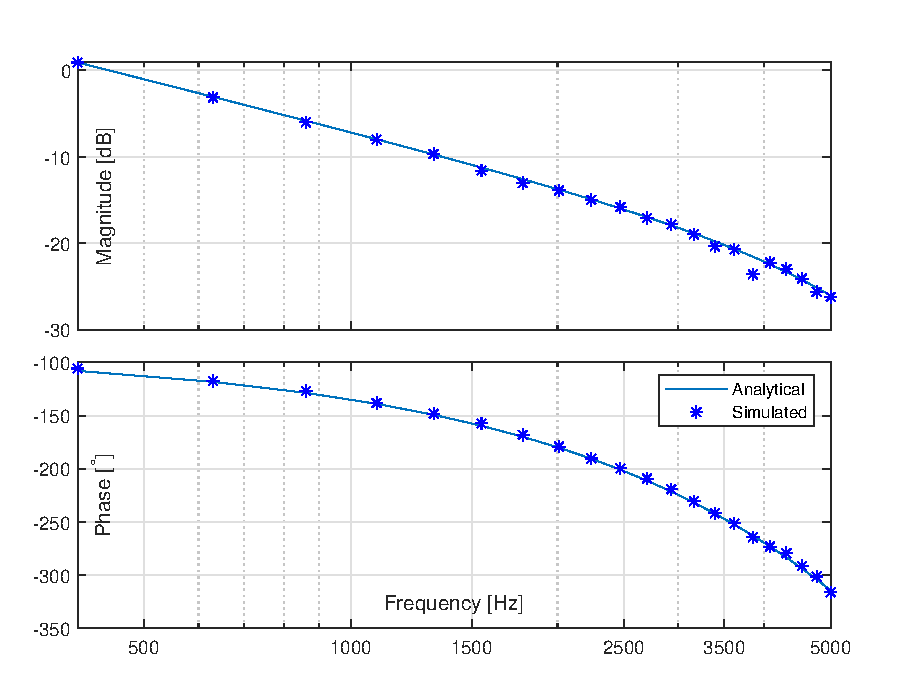
\includegraphics[width=0.95\linewidth]{figures/MSDU_olfra.eps}}
    \caption{Simulated open loop FRA results for MS-DU controller.}
    \label{fig:MSDU_olfra} 
\end{figure}

\begin{table}[h!]
			  \caption{Control loop parameters obtained in simulations via FRA analysis}
              \label{tab:sym_param}
              \centering
              \begin{tabular}{llll}
                           \midrule\midrule
        MS-MU+MAF & label & value   & unit\\
        \midrule               
                  Cross-over frequency  & $f_{c}$ & 800 & Hz   \\
                  Phase margin  & $pm$ & 70 &  $^\circ$  \\
                  \midrule\midrule
        DS-DU & label & value   & unit\\
        \midrule               
                  Cross-over frequency  & $f_{c}$ & 800 & Hz   \\
                  Phase margin  & $pm$ & 68.254 &  $^\circ$  \\
                  \midrule\midrule
        MS-DU & label & value   & unit\\
        \midrule               
                  Cross-over frequency  & $f_{c}$ & 550 & Hz   \\
                  Phase margin  & $pm$ & 65.181 &  $^\circ$  \\
                  \midrule\midrule
                                                        
              \end{tabular}
\end{table}

\section{Further steps before publication}
The steps are sorted from most important to less important.
\begin{itemize}
\item{Experimental verification for all regimes tested in simulations, on f28379d DSP platform. It is important to obtain results on a standard, industrial DSP. f28335 is also an option, however it has lower CPU frequency, so I am not sure we would be able to get entire FOC with N =8. The entire code for f28379d is already made, and tested in HIL simulations, so we are sure that the method works properly.}
\item{Experimental veryfication of improvement obtained regarding jittering suppression. Motor currents should have much lower noise floor in multisampled case!}
\item{Also, from experimental setup, it will be possible to see how does controller behave with multisampled control, without MAFs (perhaps just with some weaker digital filters). In simulations, it was working very well, but there we do not have switching noise due to high dV/dT.}
\item{Perhaps, add part where phase lag due to MAF is compensated using proportional-derivative action, as in [10.1109/JESTPE.2018.2888980].}
\end{itemize}

\section{Conclusion}
Nothing yet.

\ifCLASSOPTIONcaptionsoff
  \newpage
\fi

\bibliographystyle{IEEEtran}
% argument is your BibTeX string definitions and bibliography database(s)
\bibliography{IEEEabrv,bib/mybibliography.bib}

\end{document}



